\documentclass[10pt,pagesize]{scrbook}

\usepackage{tikz}
% \tikzset{font=\small}
% \tikzset{every node/.append style={transform shape=false}}
% \makeatletter
% \tikzset{ScalePlotMarksOff/.code={
%         \def\pgfuseplotmark##1{\pgftransformresetnontranslations\csname pgf@plot@mark@##1\endcsname}
% }}
% \makeatother

\usepackage{pgfplots}
% \pgfplotsset{compat=1.10}
% \usetikzlibrary{arrows,positioning}
% \tikzset{font=\small}
% \tikzset{every node/.append style={transform shape=false}}

\begin{document}

\thispagestyle{empty}

\begin{figure}[htb]
  \centering
  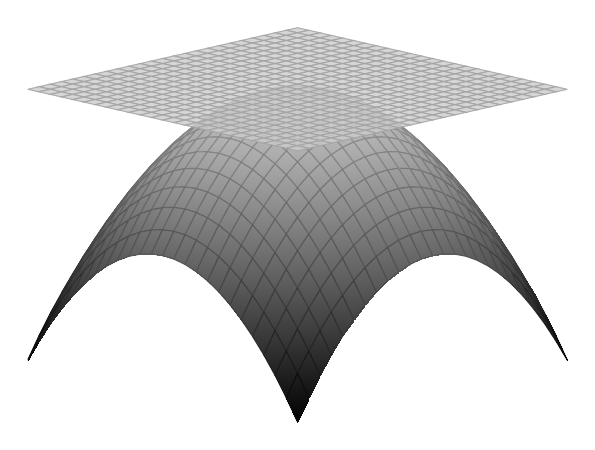
\begin{tikzpicture} 
  \begin{axis}[ view/az=45,
    view/el=15,
    axis lines=none,
    colormap={bw}{gray(0cm)=(0); gray(1cm)=(0.8)}]
    \addplot3[surf,domain=-1:1,y domain=-1:1, shader=faceted interp] {-(x^2+y^2)};
    \addplot3[surf,domain=-1:1,y domain=-1:1,opacity=.8] {0};    
  \end{axis} 
\end{tikzpicture}

  % \caption{}\label{fig:10.3}
\end{figure}

\end{document}
